\documentclass{standalone}
\usepackage{tikz}
\usetikzlibrary{patterns, positioning}
\usepackage[sfdefault]{ClearSans} %% option 'sfdefault' activates Clear Sans as the default text font
\usepackage[T1]{fontenc}

\begin{document}
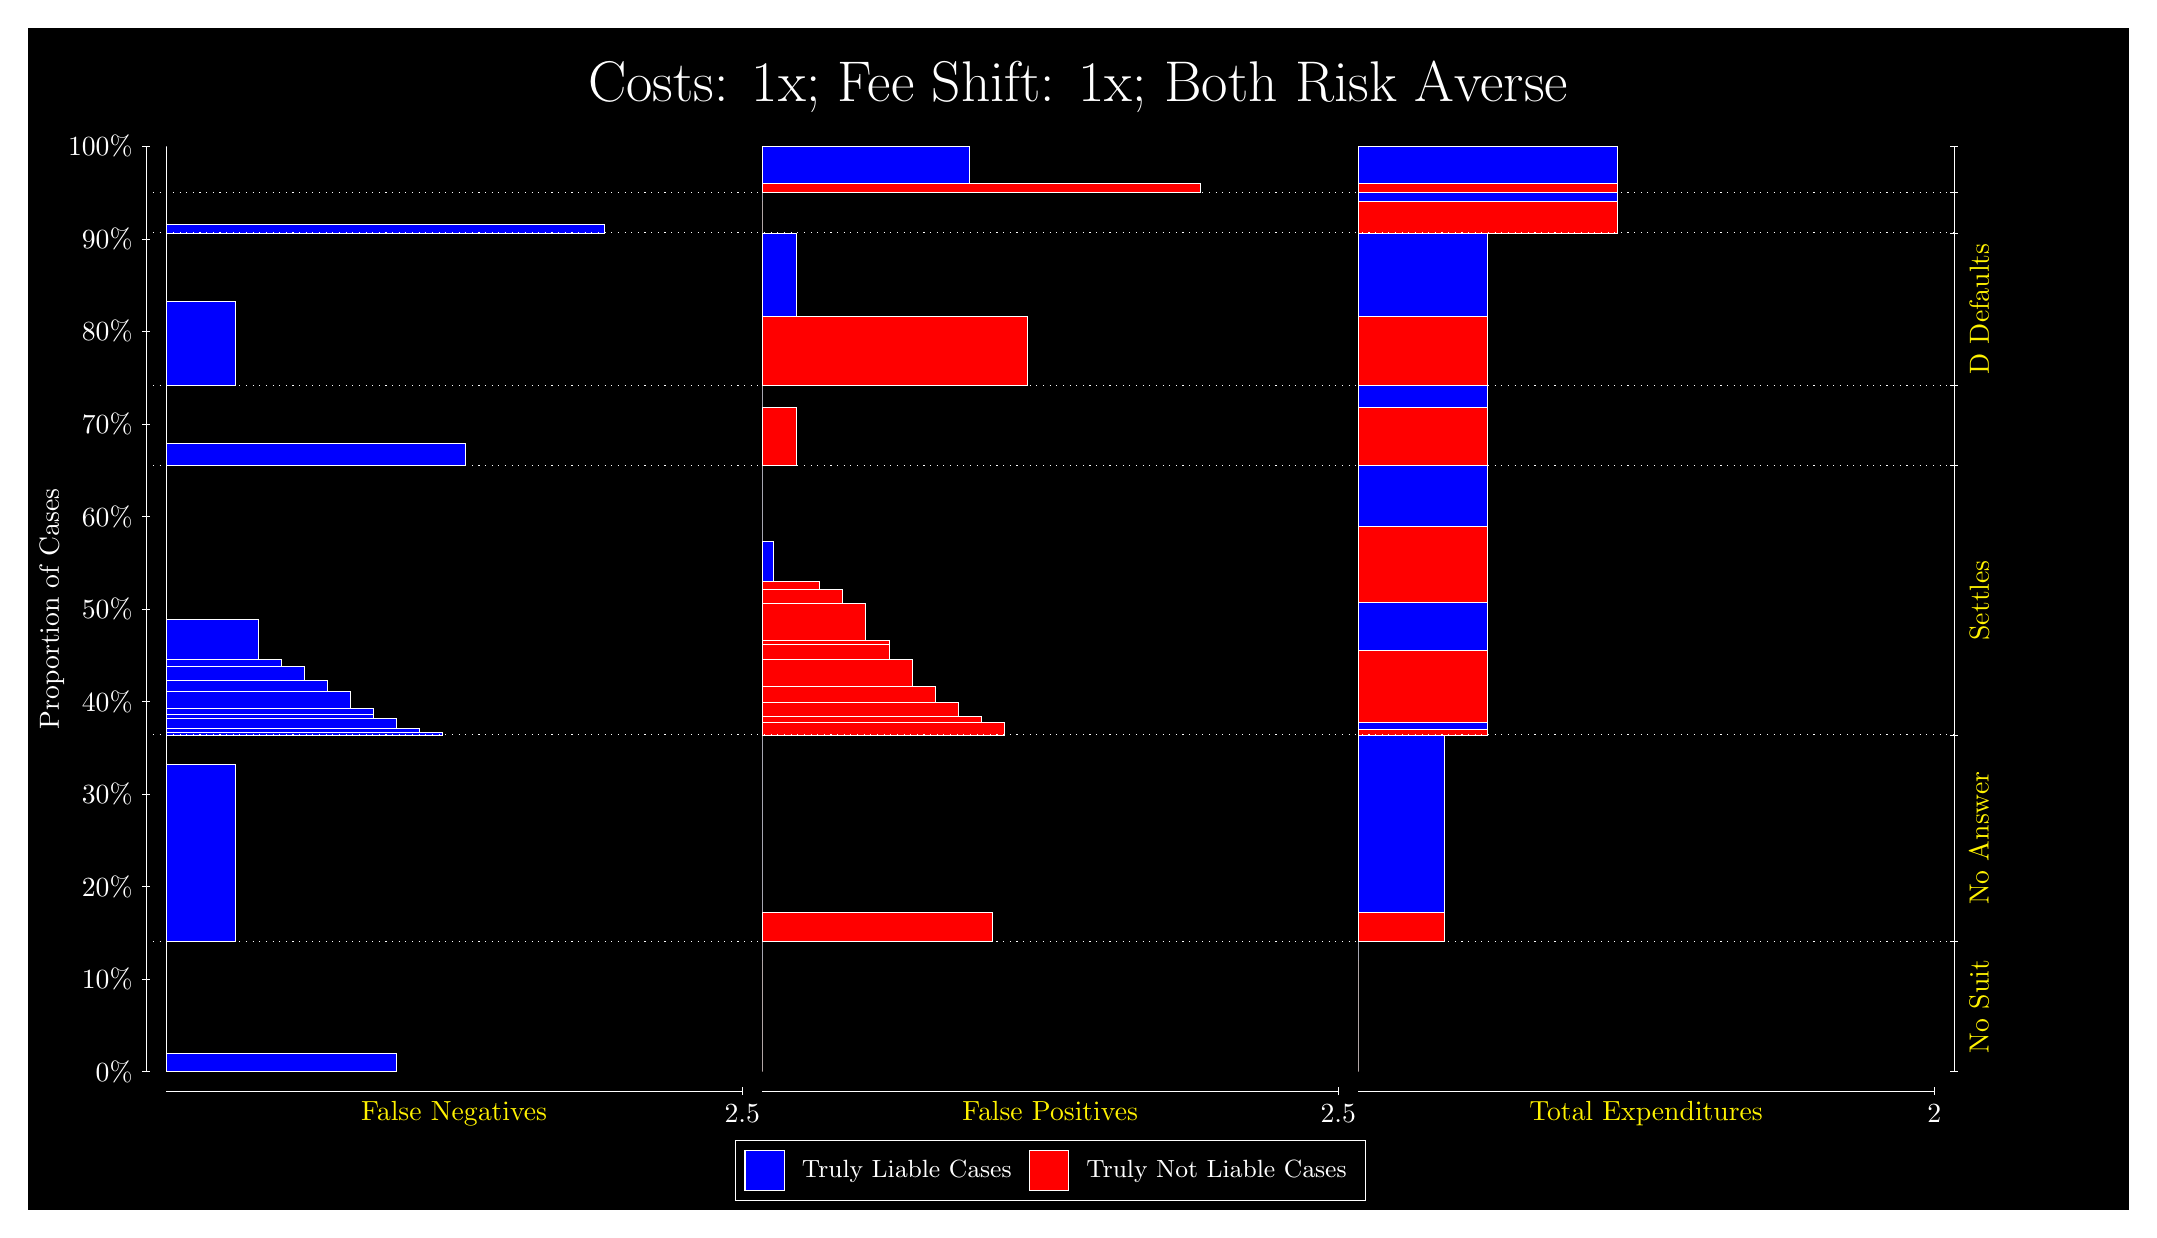
\begin{tikzpicture}
\draw[fill=black] (0,0) rectangle (26.667,15);
\draw[text=white] (0,13.5) rectangle (26.667,15) node[midway] {\huge Costs: 1x; Fee Shift: 1x; Both Risk Averse};
\draw[white, very thin] (1.5,1.75) -- (1.5,13.5);
\node[rotate=90, text=white, anchor=center] at (0.3, 7.625) {Proportion of Cases};
\draw[white, very thin] (1.45,1.75) -- (1.55,1.75);
\node[text=white, anchor=east] at (1.45, 1.75) {0\%};
\draw[white, very thin] (1.45,2.925) -- (1.55,2.925);
\node[text=white, anchor=east] at (1.45, 2.925) {10\%};
\draw[white, very thin] (1.45,4.1) -- (1.55,4.1);
\node[text=white, anchor=east] at (1.45, 4.1) {20\%};
\draw[white, very thin] (1.45,5.275) -- (1.55,5.275);
\node[text=white, anchor=east] at (1.45, 5.275) {30\%};
\draw[white, very thin] (1.45,6.45) -- (1.55,6.45);
\node[text=white, anchor=east] at (1.45, 6.45) {40\%};
\draw[white, very thin] (1.45,7.625) -- (1.55,7.625);
\node[text=white, anchor=east] at (1.45, 7.625) {50\%};
\draw[white, very thin] (1.45,8.8) -- (1.55,8.8);
\node[text=white, anchor=east] at (1.45, 8.8) {60\%};
\draw[white, very thin] (1.45,9.975) -- (1.55,9.975);
\node[text=white, anchor=east] at (1.45, 9.975) {70\%};
\draw[white, very thin] (1.45,11.15) -- (1.55,11.15);
\node[text=white, anchor=east] at (1.45, 11.15) {80\%};
\draw[white, very thin] (1.45,12.325) -- (1.55,12.325);
\node[text=white, anchor=east] at (1.45, 12.325) {90\%};
\draw[white, very thin] (1.45,13.5) -- (1.55,13.5);
\node[text=white, anchor=east] at (1.45, 13.5) {100\%};

\draw[white, very thin] (24.457,1.75) -- (24.457,13.5);
\draw[white, very thin] (24.407,1.75) -- (24.507,1.75);
\node[anchor=west] at (24.407, 1.75) {};
\draw[white, very thin] (24.407,3.4001) -- (24.507,3.4001);
\node[anchor=west] at (24.407, 3.4001) {};
\draw[white, very thin] (24.407,6.0246) -- (24.507,6.0246);
\node[anchor=west] at (24.407, 6.0246) {};
\draw[white, very thin] (24.407,9.4431) -- (24.507,9.4431);
\node[anchor=west] at (24.407, 9.4431) {};
\draw[white, very thin] (24.407,10.468) -- (24.507,10.468);
\node[anchor=west] at (24.407, 10.468) {};
\draw[white, very thin] (24.407,12.4) -- (24.507,12.4);
\node[anchor=west] at (24.407, 12.4) {};
\draw[white, very thin] (24.407,12.919) -- (24.507,12.919);
\node[anchor=west] at (24.407, 12.919) {};
\draw[white, very thin] (24.407,13.5) -- (24.507,13.5);
\node[anchor=west] at (24.407, 13.5) {};

\draw[white, very thin, fill=blue] (1.75,1.75) rectangle (4.6775,1.9863);
\draw[white, very thin, fill=red] (1.75,1.9863) rectangle (1.75,3.4001);
\draw[white, very thin, fill=blue] (1.75,3.4001) rectangle (2.6283,5.6467);
\draw[white, very thin, fill=red] (1.75,5.6467) rectangle (1.75,6.0246);
\draw[white, very thin, fill=blue] (1.75,6.0246) rectangle (5.2631,6.0557);
\draw[white, very thin, fill=blue] (1.75,6.0557) rectangle (4.9703,6.1068);
\draw[white, very thin, fill=blue] (1.75,6.1068) rectangle (4.6775,6.2417);
\draw[white, very thin, fill=blue] (1.75,6.2417) rectangle (4.3848,6.2808);
\draw[white, very thin, fill=blue] (1.75,6.2808) rectangle (4.3848,6.359);
\draw[white, very thin, fill=blue] (1.75,6.359) rectangle (4.092,6.5762);
\draw[white, very thin, fill=blue] (1.75,6.5762) rectangle (3.7993,6.7248);
\draw[white, very thin, fill=blue] (1.75,6.7248) rectangle (3.5065,6.8956);
\draw[white, very thin, fill=blue] (1.75,6.8956) rectangle (3.2138,6.9812);
\draw[white, very thin, fill=blue] (1.75,6.9812) rectangle (2.921,7.4932);
\draw[white, very thin, fill=red] (1.75,7.4932) rectangle (1.75,9.4431);
\draw[white, very thin, fill=blue] (1.75,9.4431) rectangle (5.5558,9.7252);
\draw[white, very thin, fill=red] (1.75,9.7252) rectangle (1.75,10.468);
\draw[white, very thin, fill=blue] (1.75,10.468) rectangle (2.6283,11.528);
\draw[white, very thin, fill=red] (1.75,11.528) rectangle (1.75,12.4);
\draw[white, very thin, fill=blue] (1.75,12.4) rectangle (7.3123,12.516);
\draw[white, very thin, fill=red] (1.75,12.516) rectangle (1.75,12.919);
\draw[white, very thin, fill=red] (1.75,12.919) rectangle (1.75,13.036);
\draw[white, very thin, fill=blue] (1.75,13.036) rectangle (1.75,13.5);
\draw[white, very thin, fill=red] (9.3189,1.75) rectangle (9.3189,3.1639);
\draw[white, very thin, fill=blue] (9.3189,3.1639) rectangle (9.3189,3.4001);
\draw[white, very thin, fill=red] (9.3189,3.4001) rectangle (12.246,3.7781);
\draw[white, very thin, fill=blue] (9.3189,3.7781) rectangle (9.3189,6.0246);
\draw[white, very thin, fill=red] (9.3189,6.0246) rectangle (12.393,6.1865);
\draw[white, very thin, fill=red] (9.3189,6.1865) rectangle (12.1,6.2616);
\draw[white, very thin, fill=red] (9.3189,6.2616) rectangle (11.807,6.4387);
\draw[white, very thin, fill=red] (9.3189,6.4387) rectangle (11.515,6.6372);
\draw[white, very thin, fill=red] (9.3189,6.6372) rectangle (11.222,6.9802);
\draw[white, very thin, fill=red] (9.3189,6.9802) rectangle (10.929,7.1753);
\draw[white, very thin, fill=red] (9.3189,7.1753) rectangle (10.929,7.2218);
\draw[white, very thin, fill=red] (9.3189,7.2218) rectangle (10.636,7.699);
\draw[white, very thin, fill=red] (9.3189,7.699) rectangle (10.344,7.8775);
\draw[white, very thin, fill=red] (9.3189,7.8775) rectangle (10.051,7.9745);
\draw[white, very thin, fill=blue] (9.3189,7.9745) rectangle (9.4652,8.4865);
\draw[white, very thin, fill=blue] (9.3189,8.4865) rectangle (9.3189,9.4431);
\draw[white, very thin, fill=red] (9.3189,9.4431) rectangle (9.758,10.186);
\draw[white, very thin, fill=blue] (9.3189,10.186) rectangle (9.3189,10.468);
\draw[white, very thin, fill=red] (9.3189,10.468) rectangle (12.686,11.34);
\draw[white, very thin, fill=blue] (9.3189,11.34) rectangle (9.758,12.4);
\draw[white, very thin, fill=red] (9.3189,12.4) rectangle (9.3189,12.803);
\draw[white, very thin, fill=blue] (9.3189,12.803) rectangle (9.3189,12.919);
\draw[white, very thin, fill=red] (9.3189,12.919) rectangle (14.881,13.036);
\draw[white, very thin, fill=blue] (9.3189,13.036) rectangle (11.954,13.5);
\draw[white, very thin, fill=red] (16.888,1.75) rectangle (16.888,3.1639);
\draw[white, very thin, fill=blue] (16.888,3.1639) rectangle (16.888,3.4001);
\draw[white, very thin, fill=red] (16.888,3.4001) rectangle (17.986,3.7781);
\draw[white, very thin, fill=blue] (16.888,3.7781) rectangle (17.986,6.0246);
\draw[white, very thin, fill=red] (16.888,6.0246) rectangle (18.534,6.0997);
\draw[white, very thin, fill=blue] (16.888,6.0997) rectangle (18.534,6.1853);
\draw[white, very thin, fill=red] (16.888,6.1853) rectangle (18.534,7.099);
\draw[white, very thin, fill=blue] (16.888,7.099) rectangle (18.534,7.7138);
\draw[white, very thin, fill=red] (16.888,7.7138) rectangle (18.534,8.675);
\draw[white, very thin, fill=blue] (16.888,8.675) rectangle (18.534,9.4431);
\draw[white, very thin, fill=red] (16.888,9.4431) rectangle (18.534,10.186);
\draw[white, very thin, fill=blue] (16.888,10.186) rectangle (18.534,10.468);
\draw[white, very thin, fill=red] (16.888,10.468) rectangle (18.534,11.34);
\draw[white, very thin, fill=blue] (16.888,11.34) rectangle (18.534,12.4);
\draw[white, very thin, fill=red] (16.888,12.4) rectangle (20.181,12.803);
\draw[white, very thin, fill=blue] (16.888,12.803) rectangle (20.181,12.919);
\draw[white, very thin, fill=red] (16.888,12.919) rectangle (20.181,13.036);
\draw[white, very thin, fill=blue] (16.888,13.036) rectangle (20.181,13.5);
\draw[white, dotted] (1.5,3.4001) -- (24.457,3.4001);
\draw[white, dotted] (1.5,6.0246) -- (24.457,6.0246);
\draw[white, dotted] (1.5,9.4431) -- (24.457,9.4431);
\draw[white, dotted] (1.5,10.468) -- (24.457,10.468);
\draw[white, dotted] (1.5,12.4) -- (24.457,12.4);
\draw[white, dotted] (1.5,12.919) -- (24.457,12.919);
\draw[white, very thin] (1.75,1.5) -- (9.0689,1.5);
\node[text=yellow, anchor=north] at (5.4094, 1.5) {False Negatives};
\draw[white, very thin] (9.0689,1.45) -- (9.0689,1.55);
\node[text=white, anchor=north] at (9.0689, 1.45) {2.5};

\draw[white, very thin] (9.3189,1.5) -- (16.638,1.5);
\node[text=yellow, anchor=north] at (12.978, 1.5) {False Positives};
\draw[white, very thin] (16.638,1.45) -- (16.638,1.55);
\node[text=white, anchor=north] at (16.638, 1.45) {2.5};

\draw[white, very thin] (16.888,1.5) -- (24.207,1.5);
\node[text=yellow, anchor=north] at (20.547, 1.5) {Total Expenditures};
\draw[white, very thin] (24.207,1.45) -- (24.207,1.55);
\node[text=white, anchor=north] at (24.207, 1.45) {2};

\node[text=yellow, centered, rotate=90] at (24.777, 2.5751) {No Suit};
\node[text=yellow, centered, rotate=90] at (24.777, 4.7124) {No Answer};
\node[text=yellow, centered, rotate=90] at (24.777, 7.7339) {Settles};

\node[text=yellow, centered, rotate=90] at (24.777, 11.434) {D Defaults};



\draw (12.978300999999998,1.5) node[draw=none] (baseCoordinate) {};
\begin{scope}[align=center]
        \matrix[scale=0.5, draw=white, below=0.5cm of baseCoordinate, nodes={draw}, column sep=0.1cm]{
            \node[rectangle, draw, minimum width=0.5cm, minimum height=0.5cm, fill=blue] {}; &
            \node[draw=none, font=\small, text=white] (B) {Truly Liable Cases}; &
            \node[rectangle, draw, minimum width=0.5cm, minimum height=0.5cm, fill=red] {}; &
            \node[draw=none, font=\small, text=white] (B) {Truly Not Liable Cases}; \\
            };
\end{scope}

\end{tikzpicture}
\end{document}